\chapter{Spécifications techniques et fonctionnelles}

    \section{Logiciel de simulation}

        La simulation de milieux marins est quelque chose de connu dans le domaine de la robotique. Il existe de nombreux simulateurs d'environnements marins et sous-marins~\cite{Manhaes_2016, bingham19toward, MARS, Rock}. Ces simulateurs proposent tous un modèle de flottabilité pour les objets à simuler, ce qui permet de pouvoir définir des bateaux ou bien des robots sous-marins. Cela permet donc de pouvoir simuler le comportement des \gls{ROV}s dans l'eau. Ils proposent ensuite différentes spécificités qui permettent d'avoir des éléments supplémentaires dans notre simulation. \textsc{UUV Simulator}~\cite{Manhaes_2016} est probablement le plus connu d'entre eux. C'est un simulateur de \gls{ROV} comportant un certain nombre d'éléments d'environnements simulés, comme des mondes marins, du courant ou des ombilicaux par exemple. Il propose aussi la description d'un bon nombre de robots sous-marins commercialisés, et la communauté active partage les nouveaux modèles régulièrement. \textsc{Mars}~\cite{MARS} est un simulateur spécifique à des robot baptisés \textsc{Mars}. \textsc{Rock-Gazebo}~\cite{Rock} est un projet d'intégration de simulateur basé sur le moteur physique \gls{Gazebo} et sur le framework\footnote{Infrastructure logicielle facilitant le développement logiciel} \textsc{Robot Construction Kit}. Le simulateur \textsc{VRX}~\cite{bingham19toward} est un projet open-source de robotique marine dont un simulateur a été implémenté sur la base de \gls{Gazebo}. Il propose un ensemble d'environnement, de modèles et de plugin permettant la simulation de missions de vaisseaux de surface, avec notamment la possibilité de prendre en compte la présence de vagues et de vent à la surface.

        Ces simulateurs proposent tous des spécificités différentes et intéressantes. Cependant, notre application de simulation de \gls{ROV}s pour \textsc{Forssea Robotics} est assez contrainte. En effet, l'existance de composants spécifiques, comme la simulation du \gls{Latch} ainsi que la \gls{frameLBL} rendent l'adaptation de simulateurs déjà existants trop difficile. C'est pourquoi il est nécéssaire de réaliser notre propre simulateur.

        En outre, l'étude de l'existant nous aura au moins permis de se rendre compte que \gls{Gazebo}~\cite{Koenig-gazebo} est largement utilisé dans le domaine de la simulation sous-marine, mais aussi plus largement dans la simulation robotique. \gls{Gazebo} est un logiciel de simulation multi-physique open-source\footnote{Code communautaire ouvert libre de redistribution et d'accès}. Il est aujourd'hui développé par la communauté \gls{OpenRobotics}. Il présente l'avantage de pouvoir communiquer avec \gls{ROS}, ce qui est une exigence importante de notre simulateur, car il doit permettre de tester l'implémentation logicielle des robots. La description des robots se fait en utilisant le language \gls{SDF}\footnote{\url{http://sdformat.org/}}, et il est possible de décrire le comportement complexe d'un composant en implémentant un \gls{Plugin}.


    \section{Spécifications techniques}

    \section{Spécifications fonctionnelles}

    \section{Architecture logicielle}

        L'exigence principale du simulateur étant de s'interfacer parfaitement avec le reste de l'implémentation logicielle, il est nécéssaire de définir une architecture logicielle permettant de communiquer à la fois avec les \gls{ROV}s réels et simulés. \gls{ROS2Control}~\cite{ros_control} est un framework permettant de faire communiquer des contrôleurs et des drivers ensemble. L'avantage est de pouvoir changer à chaud de contôleurs de manière consistante, sans temps mort durant lesquels le robot ne serait pas commandé. L'architecture de \gls{ROS2Control} permet aussi de faire des \gls{HardwareInterface} pour des actionneur et des capteurs réels ou simulés, qui sont des interface logicielle permettant de communiquer avec du matériel. En chargeant la version réelle ou simulée de l'\gls{HardwareInterface}, on est donc en mesure d'utiliser les contrôleurs sur les \gls{ROV}s réels ou simulés.

        \begin{figure}[!htb]
            \centering
            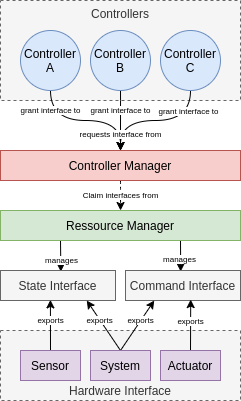
\includegraphics[width=0.5\textwidth]{imgs/ros2_control.png}
            \caption{Architecture logicielle avec \gls{ROS2Control}}
            \label{fig:ros2_control}
        \end{figure}

        La \textsc{Figure}~\ref{fig:ros2_control} nous montre l'architecture logicielle des robots utilisant \gls{ROS2Control}. Ce framework va instancier un ControllerManager qui va s'occuper de charger les contrôleurs qui seront utilisés dans le robot. Ensuite un RessourceManager va créer les interfaces qui seront utilisées par le ControllerManager et par les HardwareInterface qui sont les interfaces qui vont communiquer avec les composants. En chargeant une HardwareInterface réelle, on sera en mesure d'utiliser le composant réel, et en chargeant une HardwareInterface simulée, on pourra prendre le contrôle du composant dans la simulation. Enfin, les CommandInterface permettent d'envoyer des informations aux composants, typiquement pour commander des actionneurs, tandis que les StateInterface permettent de reçevoir des informations de la part des composants, typiquement des informations de capteurs.
        